\documentclass[xelatex,ja=standard,11pt]{bxjsarticle}
\usepackage{lmodern}
\usepackage{amssymb,amsmath}
\usepackage{ifxetex,ifluatex}
\usepackage{fixltx2e} % provides \textsubscript
\ifnum 0\ifxetex 1\fi\ifluatex 1\fi=0 % if pdftex
  \usepackage[T1]{fontenc}
  \usepackage[utf8]{inputenc}
\else % if luatex or xelatex
  \ifxetex
    \usepackage{mathspec}
  \else
    \usepackage{fontspec}
  \fi
  \defaultfontfeatures{Ligatures=TeX,Scale=MatchLowercase}
\fi
% use upquote if available, for straight quotes in verbatim environments
\IfFileExists{upquote.sty}{\usepackage{upquote}}{}
% use microtype if available
\IfFileExists{microtype.sty}{%
\usepackage{microtype}
\UseMicrotypeSet[protrusion]{basicmath} % disable protrusion for tt fonts
}{}
\usepackage{hyperref}
\hypersetup{unicode=true,
            pdftitle={研究進捗報告},
            pdfauthor={里谷 佳紀},
            pdfborder={0 0 0},
            breaklinks=true}
\urlstyle{same}  % don't use monospace font for urls
\usepackage{graphicx,grffile}
\makeatletter
\def\maxwidth{\ifdim\Gin@nat@width>\linewidth\linewidth\else\Gin@nat@width\fi}
\def\maxheight{\ifdim\Gin@nat@height>\textheight\textheight\else\Gin@nat@height\fi}
\makeatother
% Scale images if necessary, so that they will not overflow the page
% margins by default, and it is still possible to overwrite the defaults
% using explicit options in \includegraphics[width, height, ...]{}
\setkeys{Gin}{width=\maxwidth,height=\maxheight,keepaspectratio}
\IfFileExists{parskip.sty}{%
\usepackage{parskip}
}{% else
\setlength{\parindent}{0pt}
\setlength{\parskip}{6pt plus 2pt minus 1pt}
}
\setlength{\emergencystretch}{3em}  % prevent overfull lines
\providecommand{\tightlist}{%
  \setlength{\itemsep}{0pt}\setlength{\parskip}{0pt}}
\setcounter{secnumdepth}{5}
% Redefines (sub)paragraphs to behave more like sections
\ifx\paragraph\undefined\else
\let\oldparagraph\paragraph
\renewcommand{\paragraph}[1]{\oldparagraph{#1}\mbox{}}
\fi
\ifx\subparagraph\undefined\else
\let\oldsubparagraph\subparagraph
\renewcommand{\subparagraph}[1]{\oldsubparagraph{#1}\mbox{}}
\fi

%%% Use protect on footnotes to avoid problems with footnotes in titles
\let\rmarkdownfootnote\footnote%
\def\footnote{\protect\rmarkdownfootnote}

%%% Change title format to be more compact
\usepackage{titling}

% Create subtitle command for use in maketitle
\newcommand{\subtitle}[1]{
  \posttitle{
    \begin{center}\large#1\end{center}
    }
}

\setlength{\droptitle}{-2em}
  \title{研究進捗報告}
  \pretitle{\vspace{\droptitle}\centering\huge}
  \posttitle{\par}
  \author{里谷 佳紀}
  \preauthor{\centering\large\emph}
  \postauthor{\par}
  \predate{\centering\large\emph}
  \postdate{\par}
  \date{平成29年10月31日}

\usepackage{zxjatype}
\usepackage[ipaex,scale=.95]{zxjafont}
\pagenumbering{gobble}

\begin{document}
\maketitle

\section{研究全体の目的}

深さ優先探索をベースにした,一般化ムーアグラフを発見するアルゴリズムを開発する.
さらに,初期グラフの改良や枝刈りを導入する,更なる改良案を提案する.
同時に,これらの改良を評価する.

\section{前回打ち合わせ時に定めた短期目標}

\begin{enumerate}
\def\labelenumi{\arabic{enumi}.}
\tightlist
\item
  中間報告のための資料作成
\item
  実験の継続
\item
  辺削除に対する直径の高速更新を使った探索の高速化
\item
  証明,アルゴリズムの文書化

  \begin{enumerate}
  \def\labelenumii{\alph{enumii}.}
  \tightlist
  \item
    一般化ムーアグラフの条件
  \item
    探索アルゴリズム
  \end{enumerate}
\end{enumerate}

\section{本日までの進捗状況}

\begin{enumerate}
\def\labelenumi{\arabic{enumi}.}
\tightlist
\item
  途中まで作成した.
\item
  展開グラフ数と時間の計測を,最初の一般化ムーアグラフを見つけるまでから,
  すべての一般化ムーアグラフを見つけるまでに変更して実験した.
  次数が3のときの結果を図1と 図2に示す.
\item
  未着手
\item
  一部で進捗があった.

  \begin{enumerate}
  \def\labelenumii{\alph{enumii}.}
  \tightlist
  \item
    手書きで試作した.
  \item
    前回より未着手
  \end{enumerate}
\end{enumerate}

\begin{figure}

{\centering 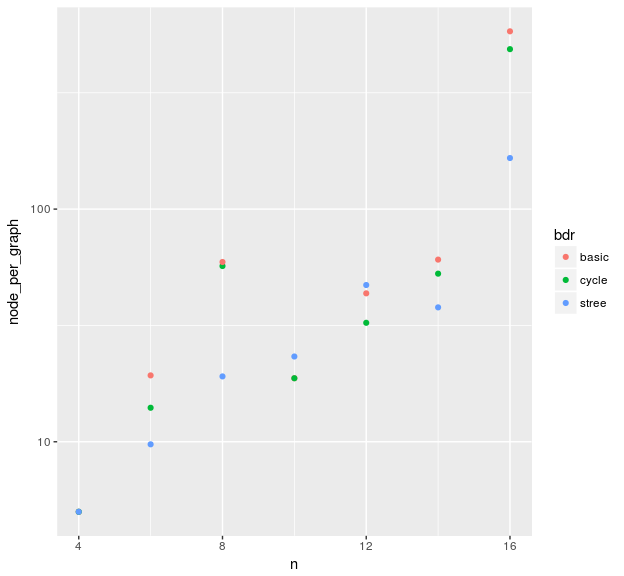
\includegraphics[width=0.7\linewidth]{week07_files/figure-latex/fig:node-full-1} 

}

\caption{発見したグラフあたりの展開グラフ数}\label{fig:fig:node-full}
\end{figure}

\begin{figure}

{\centering 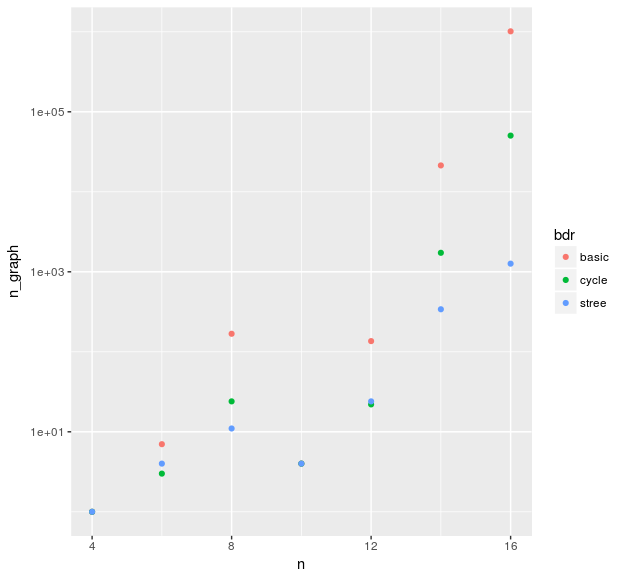
\includegraphics[width=0.7\linewidth]{week07_files/figure-latex/fig:graph-full-1} 

}

\caption{発見したグラフ数}\label{fig:fig:graph-full}
\end{figure}


\end{document}
